\documentclass[a4paper,10pt]{article}

\usepackage[T1]{fontenc}
\usepackage[sc]{mathpazo}
\linespread{1.08}
\usepackage[margin=2cm,top=1.6cm,bottom=1.8cm]{geometry}
\usepackage{graphicx}
\usepackage{amsmath,amssymb}
\usepackage{xcolor}
\usepackage{enumitem}
\usepackage{booktabs}
\usepackage{colortbl}
\usepackage{eurosym}
\usepackage{fancyhdr}
\usepackage[hidelinks]{hyperref}

\definecolor{ink}{HTML}{1A1A1A}
\definecolor{accent}{HTML}{1F4E79}
\definecolor{warm}{HTML}{B4532A}
\definecolor{quiet}{HTML}{80868B}
\definecolor{hair}{HTML}{D5D8DC}

\color{ink}
\setlist{nosep,leftmargin=1.2em,itemsep=0.3em}
\setlength{\parindent}{0pt}
\pagestyle{fancy}
\fancyhf{}
\lhead{\footnotesize\color{quiet}Use It or Lose It? \textperiodcentered{} Zheng Huang \textperiodcentered{} speaker script}
\rhead{\footnotesize\color{quiet}\thepage}
\renewcommand{\headrulewidth}{0pt}

\newcommand{\quiet}[1]{{\color{quiet}#1}}
\newcommand{\kicker}[1]{{\footnotesize\scshape\color{accent}#1}}
\newcommand{\slidepage}[2]{% #1 slide number, #2 time
  \clearpage
  \kicker{Slide #1}\hfill\quiet{\footnotesize #2}\par\smallskip
  {\setlength{\fboxsep}{0pt}\color{hair}\fbox{\includegraphics[page=#1,width=\dimexpr\textwidth-0.8pt\relax]{../slides/slides.pdf}}}\par
  \bigskip
}
\newcommand{\say}{\kicker{Say}\par\smallskip}
\newcommand{\asked}{\par\bigskip\kicker{If asked}\par\smallskip}
\newcommand{\Q}[1]{\item[\color{warm}Q] \emph{#1}}
\newcommand{\A}{\item[\color{accent}A]}

\begin{document}

% ================= COVER =================
{\color{accent}\rule{1.6cm}{1.2pt}}\par\medskip
{\fontsize{26}{30}\selectfont Use It or Lose It?}\par\smallskip
{\large\quiet{Programmable money, negative rates and the design of the digital euro}}\par\medskip
{\small Zheng Huang \textperiodcentered{} Topics of Central Banking \textperiodcentered{} October 2026}\par
{\footnotesize\quiet{Speaker script \textperiodcentered{} 20 minutes + 10 minutes Q\&A}}

\vspace{0.7cm}
\kicker{The story, slide by slide}\par\medskip
\small
\begin{enumerate}[leftmargin=2em,itemsep=0.25em]
  \item[\quiet{2}] This talk follows one question from stimulus vouchers to the design of the digital euro.
  \item[\quiet{3}] When the central bank creates money that nobody spends, monetary policy loses its grip.
  \item[\quiet{4}] Interest rates could not be cut far below zero, because cash always pays zero.
  \item[\quiet{5}] Vouchers with an expiry date get money spent, which is exactly what a liquidity trap needs.
  \item[\quiet{6}] A programmable digital euro could build this pressure into money itself, in one of two ways.
  \item[\quiet{7}] To compare the two designs, consider a holder who must search for good uses of money.
  \item[\quiet{8}] An expiry date pushes out more spending, but it ends in a fire sale and splits money into vintages.
  \item[\quiet{9}] Continuous decay keeps every euro equal, and it is nothing more than a negative interest rate.
  \item[\quiet{10}] Yet the draft regulation fixes the digital euro's interest rate at exactly zero.
  \item[\quiet{11}] A zero-rate digital euro is cash without storage costs, so it pushes the lower bound back up to zero.
  \item[\quiet{12}] The lower bound and disintermediation are the same problem: a central-bank rival to bank deposits.
  \item[\quiet{13}] A hard holding limit stops a run in a crisis, but it also blocks ordinary users in normal times.
  \item[\quiet{14}] When costs have a cliff and benefits do not, price and quantity together beat either one alone.
  \item[\quiet{15}] Each segment of the cost curve becomes one rule: a free tier, a Pigouvian rate, and a cap.
  \item[\quiet{16}] In an illustrative calibration, the rules imply a free tier of about \euro 500, a rate of about $-2.4\%$ and a cap near \euro 3{,}000.
  \item[\quiet{17}] If money is to carry a holding cost, continuous decay with a free tier and a cap is its natural form.
\end{enumerate}

\vspace{0.5cm}
\begin{minipage}[t]{0.40\textwidth}
\kicker{Timing}\par\medskip
\footnotesize
\begin{tabular}{@{}rlr@{\qquad}rlr@{}}
  1 & 0:15 & & 10 & 0:40 \\
  2 & 0:45 & & 11 & 1:10 \\
  3 & 1:15 & & 12 & 1:00 \\
  4 & 1:15 & & 13 & 1:15 \\
  5 & 1:15 & & 14 & 1:20 \\
  6 & 0:50 & & 15 & 1:30 \\
  7 & 1:15 & & 16 & 1:20 \\
  8 & 1:30 & & 17 & 1:10 \\
  9 & 1:15 & & & \\
\end{tabular}

\smallskip
\quiet{Checkpoints: end of slide 6 at 5:35; slide 9 at 9:35; slide 13 at 13:40; slide 17 at 19:00, leaving one minute of slack.}
\end{minipage}\hfill
\begin{minipage}[t]{0.55\textwidth}
\kicker{Numbers to know}\par\medskip
\footnotesize
\begin{itemize}
  \item Eurosystem balance sheet: \euro 2.2tn (2014) to \euro 8.6tn (2021); inflation below 2\% in 2014--20.
  \item Deposit facility rate $\le 0$ from June 2014 to July 2022; lowest $-0.50\%$ (2019--22).
  \item China coupons: \textyen 3 per \textyen 1. France: one-month MPC 61\% vs 23\%.
  \item Expiry vs decay, 30 days: 84\% vs 73\% useful spending; 16\% dumped; value 0.80 to 0.50.
  \item Decay of 1\% a year raises velocity by about 12\%.
  \item Art.\ 16(8): ``shall not bear interest''. Cap range \euro 1{,}500--3{,}000.
  \item Crisis outflow: \euro 699bn at \euro 3{,}000 (ECB); model \euro 648bn; no cap \euro 4.7tn.
  \item Illustration: free tier \euro 510, decay $-2.4\%$ (2.65\% $-$ 0.26\%), cap \euro 3{,}000.
  \item Appendix: design comparison (cap only 18.5\% blocked; price only \euro 4.7tn in a crisis).
\end{itemize}
\end{minipage}

% ================= SLIDES =================
\slidepage{1}{0:15}
\say
\begin{itemize}
  \item ``Good morning. My talk is about what happens if a central bank programs a holding cost into money, and what that means for the design of the digital euro.''
\end{itemize}

\slidepage{2}{0:45}
\say
\begin{itemize}
  \item ``The whole talk answers one question: should the digital euro bear interest, and in what form?''
  \item Walk down the five steps in one sentence each; tell the audience the answer comes in three numbers at the end.
\end{itemize}

\slidepage{3}{1:15}
\say
\begin{itemize}
  \item The bars are the Eurosystem balance sheet: almost four times larger in seven years.
  \item The line is inflation: below target every year until 2021.
  \item In $MV=PY$, more $M$ did not raise $PY$ because $V$ fell. People held the money.
  \item ``That is the first blockage: money is created but not spent.''
\end{itemize}
\asked
\begin{itemize}
  \Q{Wasn't the balance sheet growth meant to lower long-term rates, not to raise spending directly?}
  \A Yes, asset purchases worked through yields and portfolio rebalancing. The point is only that the extra base money did not translate into proportional spending.
\end{itemize}

\slidepage{4}{1:15}
\say
\begin{itemize}
  \item The deposit facility rate went below zero in June 2014 and stayed at or below zero for eight years.
  \item It stopped at $-0.50\%$. Below that, savers would pull money into banknotes, which pay zero.
  \item The true floor is minus the cost of holding cash: storage, insurance, transport.
  \item ``That is the second blockage: rates cannot fall far enough.''
\end{itemize}
\asked
\begin{itemize}
  \Q{Inflation is now above target. Why does this matter?}
  \A The floor was binding for most of 2009--2021, and the regulation is likely to last decades, so its design matters in both regimes.
\end{itemize}

\slidepage{5}{1:15}
\say
\begin{itemize}
  \item Governments found a way around the first blockage: vouchers with a deadline.
  \item Left: Chinese digital coupons, roughly three yuan of extra spending for each yuan of subsidy.
  \item Right: a French randomised trial; the expiry date nearly triples the one-month spending rate.
\end{itemize}
\asked
\begin{itemize}
  \Q{The Chinese coupons also had minimum-spend thresholds. Isn't that what drives the effect?}
  \A Partly, as Ding et al.\ show. That is why I add the French trial, which isolates the deadline.
\end{itemize}

\slidepage{6}{0:50}
\say
\begin{itemize}
  \item A digital euro is programmable, so a holding cost could be written into money itself.
  \item Red: an expiry date; the balance is untouched until $T$, then gone. Blue: continuous decay, Gesell's idea; a little every day.
  \item ``Same total cost, different timing. Which one should a central bank choose?''
\end{itemize}

\slidepage{7}{1:15}
\say
\begin{itemize}
  \item To answer that, I need a simple model of how holders spend.
  \item A holder searches for a good use of each euro; faster search costs more. A fire sale is always possible but worth less.
  \item The value of holding money satisfies one equation under decay and a differential equation under expiry.
  \item ``In both cases, the less money is worth holding, the faster it is spent.''
\end{itemize}
\asked
\begin{itemize}
  \Q{Why a quadratic search cost?}
  \A It is the simplest convex cost with an interior solution. With a linear cost, velocity would literally explode at the deadline; convex is the conservative case.
\end{itemize}

\slidepage{8}{1:40}
\say
\begin{itemize}
  \item Both designs are tuned to the same average velocity over 30 days, so the race is fair.
  \item Left: velocity under expiry accelerates into the deadline; under decay it is flat.
  \item Expiry gets more useful spending done, 84\% against 73\%, because it forces the whole balance out. That surprised me.
  \item But 16\% is still unspent on the last day and goes to a fire sale.
  \item Right: an expiring euro is worth 0.80 when new and 0.50 when old. One euro is no longer equal to another.
\end{itemize}
\asked
\begin{itemize}
  \Q{Why match average velocity rather than total spending?}
  \A Velocity is what the central bank wants to raise in a liquidity trap. Matching total spending is impossible, because decay always takes part of the balance.
\end{itemize}

\slidepage{9}{1:15}
\say
\begin{itemize}
  \item Decay avoids all three problems: no deadline, no fire sale, every euro worth the same.
  \item And decay at $\lambda$ is just an interest rate of $-\lambda$.
  \item The curve: velocity rises with the square root of the rate, as in Baumol--Tobin. One percent of decay, 12\% more velocity.
  \item ``Decay clears both blockages: money moves faster, and a negative rate reaches retail balances.''
\end{itemize}
\asked
\begin{itemize}
  \Q{Couldn't a smart contract simply track the age of each expiring euro?}
  \A Yes, but then shops must accept old and new euros either at par, which invites arbitrage, or at different prices, which ends the singleness of money.
\end{itemize}

\slidepage{10}{0:40}
\say
\begin{itemize}
  \item ``So the natural instrument is a rate on the digital euro. But the draft regulation rules it out.''
  \item Read the quote; point to the timeline. The text is in trilogue now, so the question is open.
\end{itemize}

\slidepage{11}{1:10}
\say
\begin{itemize}
  \item A bank cannot pay less than the best central-bank alternative, net of the cost of holding it.
  \item Cash pays zero but is costly to hold, so the floor sits at $-c$. That is why $-0.50\%$ was possible.
  \item A zero-rate digital euro pays zero and costs nothing. Up to the cap, the floor moves back to zero.
\end{itemize}
\asked
\begin{itemize}
  \Q{Retail deposit rates never went negative anyway.}
  \A For small balances banks chose not to charge. Large and corporate deposits did pay negative rates. A zero-rate digital euro turns zero into a legal floor for everyone, up to the cap.
\end{itemize}

\slidepage{12}{1:00}
\say
\begin{itemize}
  \item Left arrow: deposits flow into cash when $r_D<-c$. That is the lower bound.
  \item Right arrow: deposits flow into the digital euro when $r_D<0$. That is disintermediation.
  \item ``One mechanism, two names. And with a zero rate, the risk peaks exactly when rates are negative.''
\end{itemize}

\slidepage{13}{1:15}
\say
\begin{itemize}
  \item The ECB's current answer to disintermediation is a hard cap, around \euro 3{,}000.
  \item Left: in normal times, about 18\% of people would like to hold more; the cap simply blocks them.
  \item Right: in a crisis the cap is what matters: about \euro 0.65 trillion of outflow at \euro 3{,}000, against \euro 4.7 trillion with no cap.
  \item ``So a price seems sufficient in normal times, while in a crisis only a quantity limit works.''
\end{itemize}
\asked
\begin{itemize}
  \Q{Where does the crisis curve come from?}
  \A The ECB published \euro 156bn at a \euro 500 cap and \euro 699bn at \euro 3{,}000. I fit the survey distribution of deposits to those two points. The implied population is 360 million, close to the actual euro-area population, and the no-cap outflow of \euro 4.7tn is close to Meller and Soons' \euro 5tn.
\end{itemize}

\slidepage{14}{1:20}
\say
\begin{itemize}
  \item This is an old question: prices or quantities? Weitzman's answer depends on slopes: a price when benefits are steeper than costs, a quantity when costs are steeper.
  \item The blue staircase is the cost of deposit outflows: free, then a constant $e$, then a cliff.
  \item In normal times demand crosses the flat part, where a price works; in a crisis it hits the cliff, where only a cap works.
  \item ``Both cases sit on one curve, which points to combining the two, as Roberts and Spence showed.''
\end{itemize}
\asked
\begin{itemize}
  \Q{Hasn't Bindseil already proposed tiering?}
  \A Yes, and this builds on it. What the framework adds is a reason for each tier, from the shape of the cost curve.
\end{itemize}

\slidepage{15}{1:30}
\say
\begin{itemize}
  \item Before any numbers, the logic: each segment of the staircase turns into one rule.
  \item Segment 1, free: outflows that banks absorb at no cost. So payment balances can be free, and the tier is set so that they just fill that free capacity.
  \item Segment 2, cost $e$: each further euro costs the bank $e$ to replace. A Pigouvian rate of $-e$ makes holders bear that cost.
  \item Segment 3, the cliff: no price is high enough, so only a cap keeps crisis outflows within the buffer.
\end{itemize}
\asked
\begin{itemize}
  \Q{What does Pigouvian mean here?}
  \A A charge equal to the cost one person's choice imposes on others. Here the cost falls on banks, which must replace lost deposits with dearer funding.
\end{itemize}

\slidepage{16}{1:20}
\say
\begin{itemize}
  \item Now the numbers, as an illustration of orders of magnitude.
  \item Free tier: the ECB expects digitalisation to bring \euro 127bn of new deposits. Filling exactly that with payment balances gives a tier of about \euro 500.
  \item Rate: a bank replaces a lost deposit at the refinancing rate, 2.65\%, instead of 0.26\%; that difference is about 2.4 points.
  \item Cap: I take the outflow the ECB itself judged manageable, which brings us back to its \euro 3{,}000.
  \item ``The cap reproduces the ECB's figure; the tier and the rate depend on the model's assumptions, and the appendix shows how sensitive they are.''
\end{itemize}
\asked
\begin{itemize}
  \Q{Isn't $-2.4\%$ a very large penalty?}
  \A Almost nobody would pay it; it mainly keeps the digital euro from becoming a savings account. It is also an upper bound: if central-bank funding replaces deposits cheaply, the social cost is lower.
  \Q{Why \euro 127bn?}
  \A It is a natural benchmark: banks end up no worse off than today. With \euro 100--300bn the tier ranges from \euro 370 to \euro 1{,}840 (appendix).
  \Q{Does the hybrid actually perform better?}
  \A In the model, yes: compared with a cap alone it blocks fewer users and leaks far less when rates are negative, and unlike a price alone it holds in a crisis. The comparison is in the appendix.
\end{itemize}

\slidepage{17}{1:10}
\say
\begin{itemize}
  \item Summarise the four points in one breath each.
  \item Mention the open questions honestly: general equilibrium, the true social cost of outflows, behaviour, and legal feasibility.
  \item Close: ``The zero-rate design is a choice with a cost. My aim was to make that cost visible, and to show what form a holding cost on money would naturally take. Thank you.''
\end{itemize}
\asked
\begin{itemize}
  \Q{Should the cap move over time?}
  \A Possibly. Since the cap protects bank liquidity, it could follow a published rule tied to banks' liquidity ratios. I sketch this in the appendix, but it raises its own questions about signalling in a crisis.
\end{itemize}

% ================= Q&A + GLOSSARY =================
\clearpage
\kicker{More questions}\par\medskip
\begin{itemize}[leftmargin=1.5em,itemsep=0.6em]
  \Q{Isn't negative interest on CBDC already in Bordo and Levin (2017)?}
  \A Yes, the idea is theirs. This talk adds a comparison of expiry and decay in one model, and a framework for combining a rate with a cap; the related literature is in the appendix.
  \Q{Would people accept a digital euro that can shrink?}
  \A Balances up to the free tier never shrink. Above it, the charge only makes the digital euro no better than a bank account.
  \Q{The ECB says the digital euro will not be programmable money.}
  \A That means no restrictions on what it can buy. Decay restricts nothing; it is a rate on a balance.
  \Q{Your model is partial equilibrium.}
  \A Yes. The qualitative results do not depend on general equilibrium, and the magnitudes are calibrated to the ECB's own numbers.
  \Q{Do coupons just pull spending forward?}
  \A The evidence is mixed: Xing et al.\ (2023) find purchases moved forward, Ding et al.\ (2024) do not. The argument does not rely on it.
\end{itemize}

\vspace{0.8cm}
\kicker{Glossary}\par\medskip
\small
\begin{tabular}{@{}p{0.25\textwidth}p{0.70\textwidth}@{}}
  Velocity & Spending per unit of money per period, $V=PY/M$. \\
  MPC & Share of an extra euro spent within a period. \\
  Lower bound (ZLB / ELB) & The rate below which savers switch to cash; slightly below zero because cash is costly to hold. \\
  Demurrage / decay & A continuous charge on holding money; a negative interest rate. \\
  Singleness of money & Every form of a currency exchanges one-for-one at par. \\
  Baumol--Tobin & Inventory model of money demand; holdings fall with the square root of the holding cost. \\
  Disintermediation & Deposits leaving banks for central-bank money. \\
  Weitzman (1974) & Prices beat quantities when benefits are steeper than costs, and vice versa. \\
  Roberts--Spence (1976) & A price schedule with a quantity ceiling beats either instrument alone. \\
  Pigouvian rate & A charge equal to the cost one holder imposes on others. \\
  LCR & Liquidity coverage ratio: liquid assets over 30-day stressed outflows; minimum 100\%. \\
  MRO & Main refinancing operations rate, 2.65\% since 16 Sep 2026. \\
  Trilogue & Negotiation between Commission, Council and Parliament on EU legislation. \\
  Art.\ 16(8) & Draft regulation: ``The digital euro shall not bear interest.''
\end{tabular}

\end{document}
